% !TeX program = lualatex
% !TeX encoding = UTF-8
\documentclass[tikz,12pt]{standalone}
  \usepackage{fontspec} 
  \setmainfont{Cambria} 

\graphicspath{{../src/FYZ/img/}}
\begin{document}
\hyphenchar\font=-1
\begin{tikzpicture}
    \node[anchor=south west,inner sep=0] 
        at (0,0) {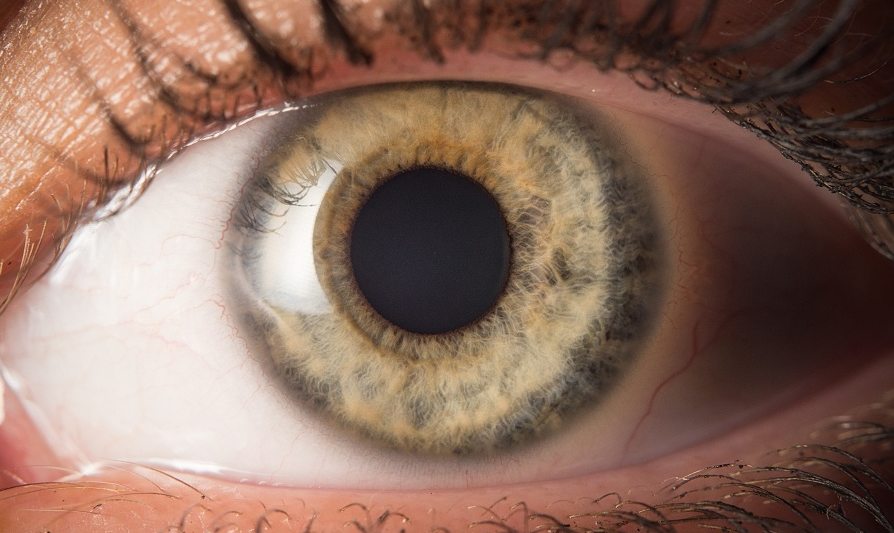
\includegraphics[width=\textwidth]{fyz_fig920.png}};
    \draw[yellow,ultra thick,->] (10,7) node[right]{Zornice, \emph{(Pupil)}} -- (7,5);
    \draw[yellow,ultra thick,->] (10,5) node[right]{Duhovka, \emph{(Iris)}} -- (8,3);
    \draw[yellow,ultra thick,->] (10,5) -- (9,5);
    \draw[black, ultra thick,->] (2,6) node[above]{Bělmo, \emph{(Sclera)}} -- (3,5);
    \draw[black, ultra thick,->] (2,6) -- (2,3);
\end{tikzpicture}
\end{document}